\documentclass[UTF8,11pt,a4paper]{ctexart}

\usepackage[a4paper,margin=2.2cm]{geometry}
\usepackage{amsmath,amssymb,mathtools,mathrsfs}
\usepackage{enumitem}
\usepackage[dvipsnames]{xcolor}
\usepackage[most]{tcolorbox}
\usepackage{fancyhdr}
\usepackage{graphicx}

\setcounter{MaxMatrixCols}{20}

\pagestyle{fancy}
\fancyhf{}
\lhead{信息理论第三次作业}
\cfoot{\thepage}
\setlength{\headheight}{14pt}

\setlist[enumerate]{leftmargin=2.2em}

\newtcolorbox{problem}[1]{
  enhanced,
  breakable,
  colback=white,
  colframe=MidnightBlue!75,
  colbacktitle=MidnightBlue,
  coltitle=white,
  boxrule=0.7pt,
  arc=1.5mm,
  left=5mm,right=5mm,top=3mm,bottom=3mm,
  title=\textbf{#1}
}

\begin{document}

\begin{center}
  {\zihao{3}\bfseries 信息理论第三次作业}\\[0.4em]
  {\small 以下各题对数均取 $\log_2$}
\end{center}

\vspace{0.8em}

\begin{problem}{4.1}
\begin{center}
  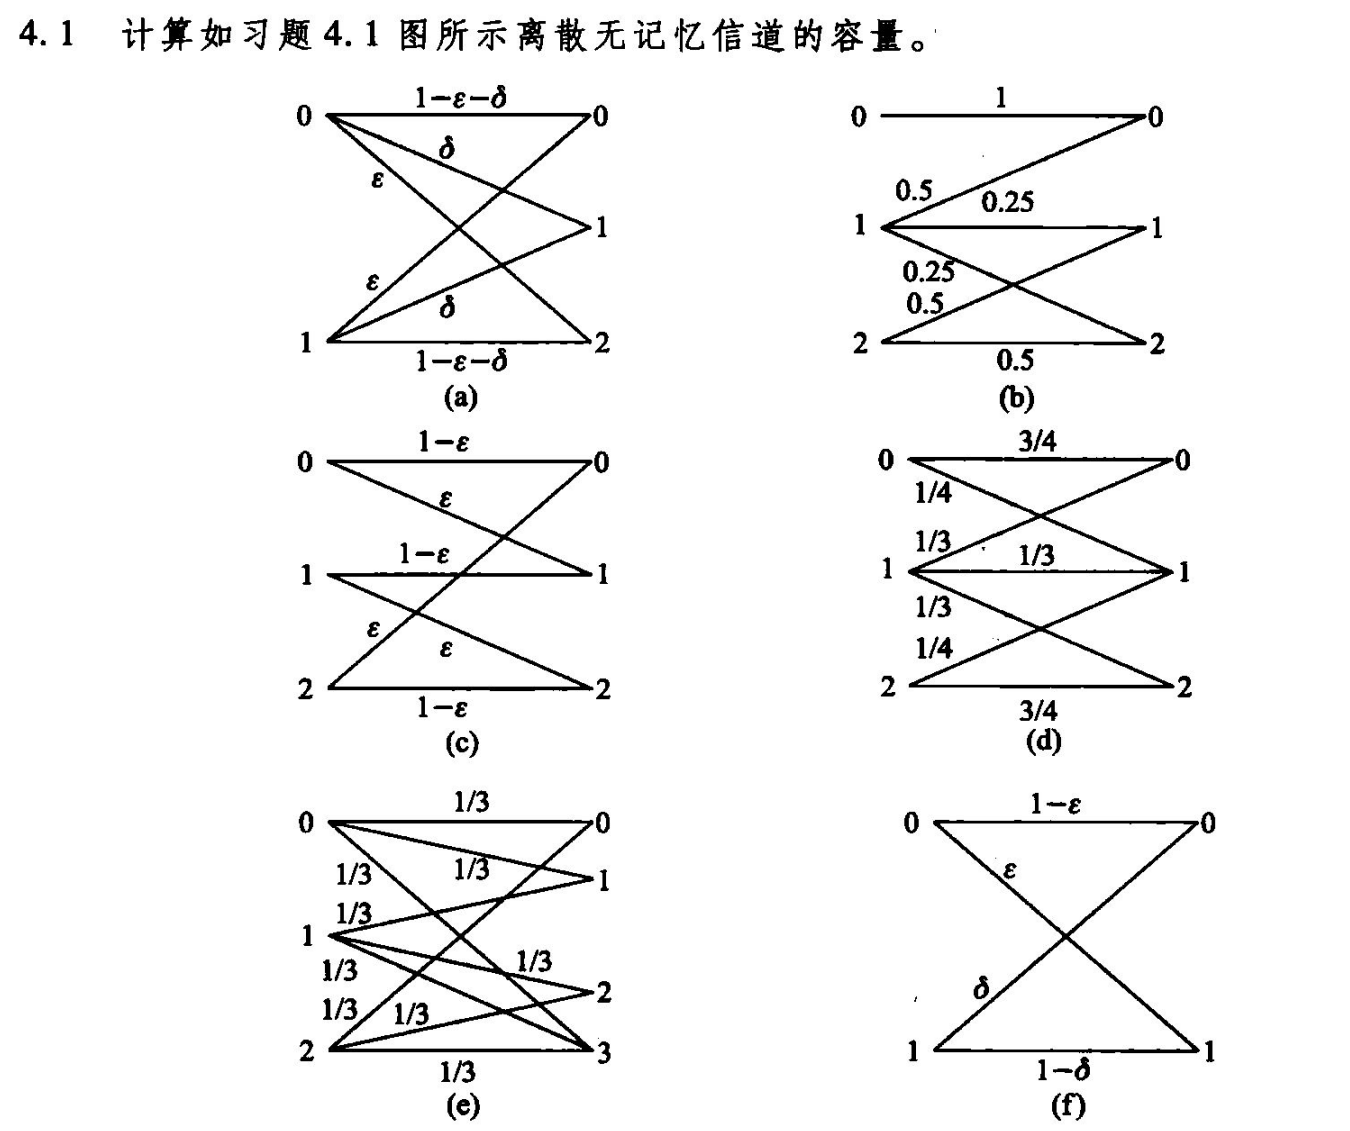
\includegraphics[width=0.85\textwidth]{assets/1.png}
\end{center}
\end{problem}
\noindent\textbf{解：}

\textbf{（a）} 信道概率转移矩阵为
\[
P = \begin{pmatrix} 1-\varepsilon-\delta & \delta & \varepsilon \\ \varepsilon & \delta & 1-\varepsilon-\delta \end{pmatrix}.
\]
信道是准对称信道，因此在输入为等概分布时达到信道容量，即 $P(X=0)=P(X=1)=0.5$ 时达到信道容量。这时
\[
P(Y=0)=0.5-0.5\delta,\quad P(Y=1)=\delta,\quad P(Y=2)=0.5-0.5\delta.
\]
相应的信道容量为
\[
C = \sum_{j=0}^{2} p(j|0)\log\frac{p(j|0)}{p(j)}
= (1-\varepsilon-\delta)\log\frac{1-\varepsilon-\delta}{0.5-0.5\delta}+\delta\log\frac{\delta}{\delta}+\varepsilon\log\frac{\varepsilon}{0.5-0.5\delta}.
\]
化简得
\[
C = (1-\varepsilon-\delta)\log(1-\varepsilon-\delta)+\varepsilon\log\varepsilon-(1-\delta)\log(0.5-0.5\delta).
\]

\textbf{（b）} 信道概率转移矩阵为
\[
P = \begin{pmatrix} 1 & 0 & 0 \\ 0.5 & 0.25 & 0.25 \\ 0 & 0.5 & 0.5 \end{pmatrix}.
\]
当 $P(X=0)=P(X=2)=0.5$，$P(X=1)=0$ 时，
\[
P(Y=0)=0.5,\quad P(Y=1)=0.25,\quad P(Y=2)=0.25.
\]
验算：
\[
I(X=0;Y)=1\ \text{bit},\quad I(X=2;Y)=0.5\log\frac{0.5}{0.25}+0.5\log\frac{0.5}{0.25}=1\ \text{bit},
\]
\[
I(X=1;Y)=0\le 1\ \text{bit}.
\]
满足达到信道容量充要条件，故
\[
C = 1\ \text{bit/次}.
\]

\textbf{（c）} 信道转移概率矩阵为
\[
P = \begin{pmatrix} 1-\varepsilon & \varepsilon & 0 \\ 0 & 1-\varepsilon & \varepsilon \\ \varepsilon & 0 & 1-\varepsilon \end{pmatrix}.
\]
信道是对称信道，当输入为均匀分布 $P(X=0)=P(X=1)=P(X=2)=\frac{1}{3}$ 时达到信道容量，
\[
C = \log 3 + \varepsilon\log\varepsilon+(1-\varepsilon)\log(1-\varepsilon) = \log 3 - H(\varepsilon).
\]

\textbf{（d）} 信道转移概率矩阵为
\[
P = \begin{pmatrix} \tfrac{3}{4} & \tfrac{1}{4} & 0 \\ \tfrac{1}{3} & \tfrac{1}{3} & \tfrac{1}{3} \\ 0 & \tfrac{1}{4} & \tfrac{3}{4} \end{pmatrix}.
\]
当 $p(X=0)=p(X=2)=0.5$，$p(X=1)=0$ 时，$P(Y=0)=P(Y=2)=\tfrac{3}{8}$，$P(Y=1)=\tfrac{2}{8}$。验算得
\[
I(X=0;Y)=I(X=2;Y)=\frac{3}{4}\ \text{bit},\quad I(X=1;Y)\le\frac{3}{4}\ \text{bit}.
\]
满足充要条件，故
\[
C = \frac{3}{4}\ \text{bit/次}.
\]

\textbf{（e）} 信道转移概率矩阵为
\[
P = \begin{pmatrix} \tfrac{1}{3} & \tfrac{1}{3} & 0 & \tfrac{1}{3} \\ \tfrac{1}{3} & \tfrac{1}{3} & \tfrac{1}{3} & 0 \\ 0 & \tfrac{1}{3} & \tfrac{1}{3} & \tfrac{1}{3} \end{pmatrix}.
\]
信道是准对称信道，当输入均匀分布 $P(X=i)=\tfrac{1}{3}$ 时达到容量。此时 $P(Y=0)=P(Y=1)=P(Y=2)=\tfrac{2}{9}$，$P(Y=3)=\tfrac{1}{3}$，故
\[
C = 6\cdot\frac{1}{9}\log\frac{1/3}{2/9}+3\cdot\frac{1}{9}\log\frac{1/3}{1/3}
= \frac{2}{3}\log\frac{3}{2}\ \text{bit/次}.
\]

\textbf{（f）} 信道转移概率矩阵为
\[
P = \begin{pmatrix} 1-\varepsilon & \varepsilon \\ \delta & 1-\delta \end{pmatrix}.
\]
利用方程求逆方法，令 $\beta_j = C+\log\omega_j$，建立方程组并求解，最终得信道容量
\[
C = \log\!\left(2^{\frac{\varepsilon H(\delta)-(1-\delta)H(\varepsilon)}{1-\delta-\varepsilon}}+2^{\frac{\delta H(\varepsilon)-(1-\varepsilon)H(\delta)}{1-\delta-\varepsilon}}\right).
\]

\vspace{0.8em}

\begin{problem}{4.2}
\begin{center}
  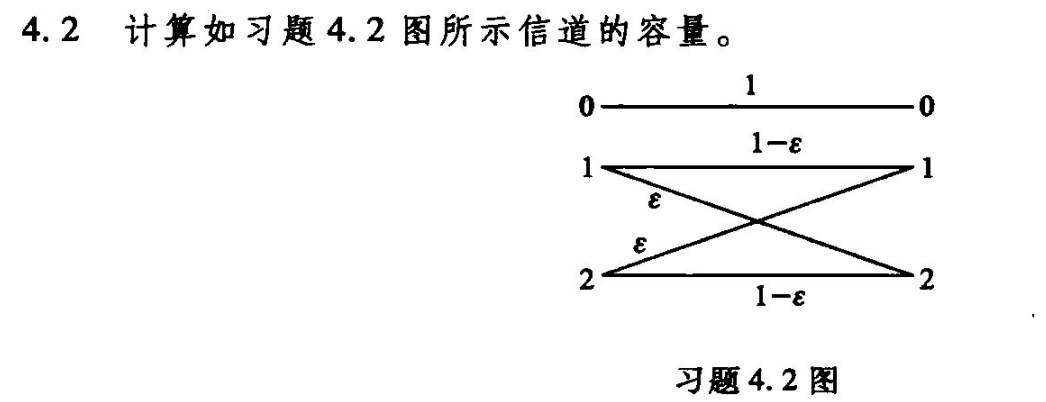
\includegraphics[width=0.75\textwidth]{assets/2.png}
\end{center}
\end{problem}
\noindent\textbf{解：}
把该信道看成是退化信道 $C_1$（输入为 $0$，输出为 $0$）和二元对称信道 $C_2$（输入为 $1,2$，输出为 $1,2$）的和信道。

退化信道容量为 $C_1=0$，二元对称信道容量为 $C_2=1-H(\varepsilon)$。

由和信道容量公式，
\[
C = \log\!\bigl[2^{C_1}+2^{C_2}\bigr] = \log\!\bigl[1+2^{1-H(\varepsilon)}\bigr].
\]
达到信道容量的输入分布为
\[
p(X=0)=\frac{2^{C_1}}{2^{C_1}+2^{C_2}}=\frac{1}{1+2^{1-H(\varepsilon)}},
\]
\[
p(X=1)=p(X=2)=\frac{2^{C_2}/2}{2^{C_1}+2^{C_2}}=\frac{2^{-H(\varepsilon)}}{1+2^{1-H(\varepsilon)}}.
\]

\vspace{0.8em}

\begin{problem}{4.9}
\begin{center}
  
\includegraphics[width=0.75\textwidth]{assets/9.png}
\end{center}
\end{problem}
\noindent\textbf{解：}
信道转移概率矩阵为
\[
P = \begin{pmatrix} p & p & 0 & 0 \\ p & p & 0 & 0 \\ 0 & 0 & p & p \\ 0 & 0 & p & p \end{pmatrix}.
\]
本信道是两个相同的二元对称信道（$\mathrm{BSC}(p)$）的和信道，每个分量信道的容量为
\[
C_1 = C_2 = 1-H(p).
\]
在输入为均匀分布时各分量信道达到容量。于是和信道容量为
\[
C = \log\!\bigl[2^{C_1}+2^{C_2}\bigr] = \log\!\bigl[2\cdot 2^{1-H(p)}\bigr] = 2-H(p)\ \text{bit/次}.
\]
相应的最佳输入分布为均匀分布：
\[
p(x_0)=p(x_1)=p(x_2)=p(x_3)=\frac{1}{4}.
\]

\end{document}
